\chapter{El juego de dominó}

\noindent

El dominó es un juego conocido alrededor de todo el mundo. Existen distintas 
modalidades de juego que varian en el número de jugadores o en las reglas para bajar una ficha.
En esta sección se define el tipo de dominó del que trata este trabajo. 
Posteriormente, se discuten algunas propiedades importantes del juego que permiten hacer 
una estimación de su complejidad y compararlo con la complejidad de otros juegos de 
mesa.

\newpage

\section{Dinámica del juego}

Para jugar se utilizan veintiocho fichas, cada una marcada con dos números entre el 
cero y el seis. Al iniciar la partida, se revuelven aleatoriamente las fichas y se reparten siete 
a cada uno de los cuatro jugadores. Los jugadores se dividen en dos equipos y se 
encuentran sentados en circulo, de tal forma que no hay dos jugadores del mismo equipo 
adyacentes.

El jugador con la ficha de dos seises es el primero en tirar y el orden de las tiradas sigue a 
la derecha. En cada turno, el jugador puede bajar una ficha si tiene algun número en común 
con los extremos externos de las fichas que ya se han jugado. El objetivo del juego es ser el 
equipo con el primer jugador que ha bajado todas sus fichas o, en caso de que ningún 
jugador pueda bajar fichas, ser el equipo cuyas fichas sumen el menor número de puntos. 

\section{Factor promedio de ramificación}

Uno de los componentes de la complejidad del juego es el número promedio de acciones que cada 
jugador puede tomar en su turno, tambien conocido como factor promedio de ramificación. 
Un cálculo analítico de este factor es dificil, pues depende de la repartición aleatoria al 
inicio del juego así como de la estrategia de cada jugador. Para obtener una estimación del 
factor se realizó la simulación de diez mil juegos con dos equipos de jugadores greedy y se 
obtuvo los siguientes resultados.

\begin{figure}[ht]
\begin{center}
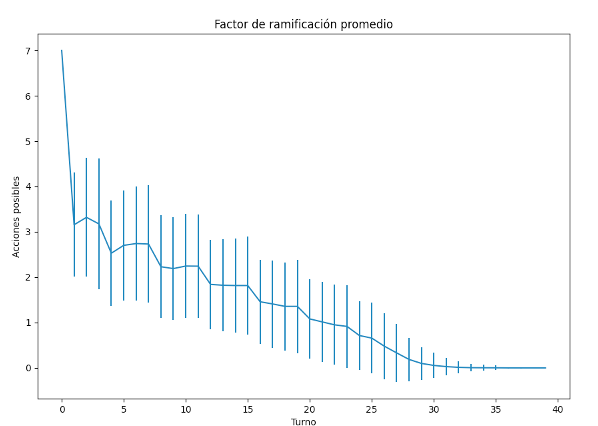
\includegraphics{factor_prom_ramificacion.png}
\caption{Factor de ramificación promedio}
\label{FPR}
\end{center}
\end{figure}

En la figura \ref{FPR} se muestra, en el eje vertical, el número promedio de fichas que un jugador 
puede tirar en el turno indicado en el eje horizontal. El primer jugador siempre puede tirar 
cualquiera de sus fichas. Después de él, los jugadores pueden tirar 3 o menos fichas en 
promedio. Este factor de ramificación es pequeño si se compara al de otros juegos de mesa 
como el ajedrez, el cual tiene un factor estimado entre 31 y 35 movimientos.

\section{Información imperfecta}

El segundo componente que influye en la complejidad del juego es la incertidumbre 
asociada a las fichas que no se conocen. Para obtener una medida de esta incertidumbre se 
calculó el número de configuraciones posibles de la información escondida. Desde la 
perspectiva del primer jugador en tirar y suponiendo que todos los jugadores bajan una 
ficha, se puede calcular el número de formas distintas en que se pueden repartir las fichas 
que no se conocen para cada vuelta del juego (cada vez que vuelve a ser turno del primer 
jugador ) y se obtuvo la siguiente tabla.

\begin{table}[H]
\centering
\caption{Posibles configuraciones de las fichas que no se conocen}
\label{PC}
\begin{tabular}{|c|c|}
\hline
 Vuelta & Posibles formas de repartir las fichas desconocidas\\ 
\hline
1 & 400 millones \\
2 & 17 millones \\
3 & 750 mil \\
4 & 34 mil \\
5 & 1600 \\
6 & 90 \\
7 & 6 \\
\hline
\end{tabular}

% \begin{tabular}{c}
% \footnotesize{Fuente: Bojilov y Phelps (2012).}
% \end{tabular}

\end{table}

Tomando en cuanta ambos componentes de la complejidad, se concluye que la 
incertidumbre asociada a la información imperfecta en las primeras vueltas del juego 
muestra ser el mayor reto a superar. 

% \subsection{Cambios cerebrales y genéticos}

% \noindent Brizendine (2010) escribe que algunos científicos piensan que ciertas áreas del cerebro son como centros de actividad que mandan señales eléctricas a otras áreas del cerebro ocasionando un determinado comportamiento.\footnote{ Por ejemplo, en el hombre la corteza del cíngulo anterior pesa opciones, detecta conflicto y motiva decisiones. La unión temporoparietal busca soluciones rápidas y ante situaciones estresantes toma en cuenta la perspectiva de otros individuos. La corteza cingulada anterior rostral se encarga de procesar los errores sociales, como la aprobación o desaprobación de otros.}

% \begin{quote}
%     \small{Mientras que la distinción entre los cerebros de niños y niñas empieza biológicamente, estudios recientes muestran que es \textit{solo} el comienzo. La estructura cerebral no está escrita sobre piedra en el nacimiento ni al final de la infancia, como antes se creía, sino que continúa cambiando a lo largo de la vida. Más que ser inmutable, nuestros cerebros son mucho más plásticos y cambiables de lo que los científicos creían hace una década. El cerebro humano es también la máquina de aprendizaje más talentosa que conocemos. Así que nuestra cultura y el cómo nos enseñaron a comportarnos desempeñan un papel importante en el diseño y reestructura de nuestros cerebros (Brizendine 2010, 5-6).}
% \end{quote}

% % Para citas muy largas es mejor el \begin{quote}

% \vspace{1em}
% \noindent \textbf{Hipótesis 3.} \hfill\begin{minipage}{\dimexpr\textwidth-3cm}
% \textit{La intensidad religiosa está relacionada negativamente con la innovación.}
% \end{minipage}
% \vspace{1em}

% Para plantear hipótesis


% Para diseñar tablas
